\chapter{Omega 3 Diet in Schizophrenia}
\section{Introduction}
As research in \glng{scz} progress, we start to identify an increasing amount of variants. 
There are now 108 variants identified to be associated with \glng{scz} \citep{Ripke2013}.
However, most of these variants only explained for a small portion of the heritability.
Using \gls{ldsc} and \gls{shrek}, we estimated the \gls{pgc} \glng{scz} \gls{GWAS} only accounts for no more than 20\% of the heritability, much least than what was estimated from the twin studies \citep{Lichtenstein2009,Sullivan2003}.
Although the \gls{pgc} \glng{scz} \gls{GWAS} bring great promises to the field of \glng{scz} genetics, there is still a long way before one can translate the findings from the \gls{pgc} \glng{scz} \gls{GWAS} into clinical applications.

Another direction of \glng{scz} research was to investigate how different environmental risk factors contribute to the etiology of \glng{scz}.
Of all the non-genetic risk factors, prenatal infection has the largest effect size \citep{Sullivan2005}.
Because of its important in \glng{scz}, prenatal infection has been extensively studied.

Early studies of prenatal infection in \glng{scz} mainly relies on ecological data such as influenza epidemics in the population to define the exposure status \citep{Brown2010}.
The problem of these studies was that the exposure status was based solely on whether an individual was in gestation at the time fo the epidemic without any confirmation of maternal infection during pregnancy.
This leads to difficulties in replication of the findings.
Subsequently, researchers uses birth cohorts where infection was documented using different biomarkers during pregnancies to provide a better labeling of the exposure status \citep{Brown2010}.
Through these rigorous studies it was found that the risk of \glng{scz} increases as long as an individual's mother was infected by different form of infectious agents such as influenza, HSV-2 and \textit{T.gondii} during gestation \citep{Brown2010}.
As different infectious agents all increase the risk of \glng{scz}, it leads to the hypothesis of \gls{mia} \citep{Brown2010} where it was hypothesized that instead of a particular infectious agents, it was the maternal immune response that disrupt the brain development in the offspring, thus leading to an elevated risk of \glng{scz}.

To really understand how \gls{mia} increase the risk of \glng{scz}, it is important to understand the molecular mechanism.
A great challenge in the study of \gls{mia} was that one cannot carry out empirical experimental design in human samples due to ethical issues.
Thus a popular alternative is to employ rodent models.
However, unlike physiological traits, psychiatric disorder such as that of \glng{scz} often contain symptoms related to higher level functioning such as hallucinations, delusion, disorganized speech etc \citep{AmericanPsychiatricAssociation2013}.
This raise challenge in diagnosing whether if the rodent has demonstrated the symptoms of \glng{scz} for not only it was difficult to check whether if the high level functioning of the rodent is disrupted, there were no available biomarkers for \glng{scz}.
Thus instead of labeling whether if the rodent is ``schizophrenic'' or ``normal'', one would rather consider whether if the rodent demonstrate any ``schizophrenia-like'' behaviours such as impaired prepulse inhibition, impaired working memory and reduced social interaction \citep{Meyer2007a}.
An important point to note here is that as autism and \glng{scz} shares most of these phenotypes, and that risk of autism is also increased in patients whose mother were exposed to infections during gestation \citep{Brown2012}, studies using these rodent models to study effect of prenatal infection were usually non-specific to \glng{scz} or autism. 
Rather, they should be considered together. 
For simplicity and focus of the current thesis, we would limit our discussion to \glng{scz}.

Recent studies of global gene expression patterns in MIA-exposed rodent fetal brains \citep{Oskvig2012,Garbett2012a} suggest that the post-pubertal onset of schizophrenic and other psychosis-related phenotypes might stem from attempts of the brain to counteract the environmental stress induced by MIA during its early development \citep{Garbett2012a}. 
To date, all these studies have focused on the changes elicited by a mid-to-late gestation exposure (e.g. \gls{gd} 12.5 for mouse, or \gls{gd} for rat). 
However, although \citet{Meyer2007a,Li2009c,Li2010a} have reported that \gls{mia} early in gestation event might exert a more extensive impact on the phenotype of offspring, the effect of early \gls{mia} on gene expression in brain of adult offspring have not been examined.
It is therefore interesting to study the gene expression changes in adult offspring who were exposed to \gls{mia} during early gestation.

Ultimately, one would like to identify treatments / cures for \glng{scz} thus help to boost the quality of life of the \glng{scz} patients.
One candidate is the n-3 \gls{pufa} which can inhibits the production of \gls{il6} \citep{Trebble2003}, a major mediator in \gls{mia} \citep{Smith2007}.
n-3 \gls{pufa} is also plays a critical role in the development of central nervous system \citep{Clandinin1999} and it has robust anti-inflammatory properties \citep{Trebble2003}.
Previous study from our lab suggested that a n-3 \gls{pufa} rich diet can help to reduce the schizophrenia-like phenotype in mouse exposed to early \gls{mia} insults \citep{Li2015}. 
Thus we would also like assess the effect of an n-3 \gls{pufa} rich diet on the gene expression pattern in the brain of the adult offspring.

% Cerebellum
Herein, we introduce a pilot study aiming to study the gene expression changes induced by early \gls{mia} exposure in the brain of the adult offspring and also expression changes induced by n-3 \gls{pufa} rich diet using RNA Sequencing - an approach considered to be more accurate and reliable compared to conventional microarrays \citep{Wang2009d}.
Moreover, RNA Sequencing are more flexible when compared to microarrays in that it can also detect alternative splicings and novel transcripts. 
Although we don't have sufficient sample size for such analysis in our pilot study, the use of RNA Sequencing allow subsequent replication studies to incorporate the pilot samples for such analysis, thus potentially reducing the cost of experiment.

Brain is a complex organ in that it is subdivided into multiple regions, each with their own responsibility.
Thus it is expected that the gene expression pattern differs from region to regions.
It is then important for us to select a region of interest for our analysis. 
Typically, 



\section{Methodology}
\subsection{Sample Preparation}
%TODO talk about the sex problem
Female and male C57BL6/N mice were bred and mated by The University of Hong Kong, Laboratory Animal Unit. 
Timed-pregnant mice were held in a normal light–dark cycle (light on at 0700 hours), and temperature and humidity-controlled animal vivarium. 
All animal procedures were approved by the Committee on the Use of Live Animals in Teaching and Research (CULATR) at The University of Hong Kong.

The MIA model was generated following procedures previously reported \citep{Li2009c}. 
A dose of 5mg kg$^{-1}$ \gls{polyic} in an injection volume 5ml kg$^{-1}$, prepared on the day of injection was administered to pregnant mice on \gls{gd} 9 via the tail vein under mild physical constraint. 
Control animals received an injection of 5ml kg$^{-1}$ 0.9\% saline. 
The animals were returned to the home cage after the injection and were not disturbed, except for weekly cage cleaning.
The resulting offspring were weaned and sexed at postnatal day 21. 
The pups were weighed and littermates of the same sex were caged separately, with three to four animal per cage.
Half of the animal were fed on diets enriched with n-3 PUFAs (Omega 3 rich) and half were fed a standard (control, Omega 6 rich) lab diet until the end of the study.
The latter `n-6 PUFA' control diet had the same calorific value and total fat content as the n-3 PUFA diet. 
The diets were custom prepared and supplied by Harlan Laboratories (Madison, WI, USA). 
The n-6 and n-3 PUFAs were derived from corn oil or menhaden fish oil, respectively. 
The n-6 PUFA control diet, was based on the standard AIN-93G rodent laboratory diet \citep{Reeves1993}, and contained 65 g kg$^{-1}$ corn oil and 5 g kg$^{-1}$ fish oil with an approximate (n6)/(n3) ratio of 13:1. 
The n-3 PUFA diet contained 35 g kg$^{-1}$ corn oil and 35 g kg$^{-1}$ fish oil with an approximate (n6)/(n3) ratio of 1:1 \citep{Olivo2005}.
The male offspring were sacrificed by cervical dislocation on postnatal week 12 and the cerebellum was extracted and stored in -80$^{\circ}$C until RNA extraction.


\subsection{RNA Extraction, Quality Control and Sequencing}
Total RNA was extracted from each cerebellum tissue using RNeasy midi kit (Qiagen) following the manufacturer's instructions.
RNA quality was assayed using the Agilent 2100 Bioanalyzer and RNA was quantified using Qubit 1.0 Flurometer.
Samples with \gls{rin} $<7$ were not included in our study as the RNA are most likely degraded.
As a pilot study, we select a minimum of 3 samples per group and each samples must come from a different litter to control for littering effect.
The RNA Sequencing library was performed at the Centre for Genomic Sciences, the University of Hong Kong, using the KAPA Strannder mRNA-Seq Kit. 
All samples were sequenced using Illumina HiSeq 1500 at 2 lanes (2x101bp paired end reads).
We distribute the samples such that each lane contain roughly the same amount of samples from different conditions.
\begin{table}
	\centering
	\begin{tabular}{rrrrrrr}
		\toprule
		SampleID & Litter & Diet & Condition & Lane & Batch & Rin\\
		\midrule
		B1&	3&	O3&	POL&	1&	B&	7.7\\
		B2&	6&	O3&	POL&	2&	B&	7.7\\
		F1&	4&	O3&	POL&	1&	F&	7.6\\
		F4&	1&	O3&	SAL&	2&	F&	8.1\\
		B4&	5&	O3&	SAL&	1&	B&	7.8\\
		B5&	14&	O3&	SAL&	2&	B&	7.7\\
		F2&	2&	O6&	POL&	1&	F&	7.5\\
		E3&	11&	O6&	POL&	2&	E&	7.8\\
		C2&	7&	O6&	POL&	2&	C&	7.9\\
		B6&	13&	O6&	SAL&	2&	B&	7.4\\
		E6&	14&	O6&	SAL&	1&	E&	8\\
		C6&	1&	O6&	SAL&	1&	C&	7.8\\
		\bottomrule
	\end{tabular}
	\caption[Sample Information]{
		Sample information.
		O3 = Omega 3 diet; O6 = Omega 6 diet; POL = \gls{polyic} exposed; SAL = Saline exposed.
		We have tried to separate the samples into different lane and batch to control for the lane and batch effect. 
		Samples from different litters were also used with the exception of 1M\_2 and 1M\_3 which came from the same litter but were given a different diet.
	}
\end{table}
\subsection{Sequencing Quality Control}
\Gls{qc} of the RNA Sequencing read data were rather standardized where FastQC \citep{Andrews2010} is the most widely adopted tools.
It can generate the required per base \gls{qc} and provide a general picture of how well the sequencing were done.

From the FastQC report, it was noted that some adapter sequences remained in the final sequence, by using trim\_glore, a wrapper for cutadapt (version 1.9.1) \citep{Martin2011}, we trim the adapter sequences from the sequence and only retain reads that were at least 75 \gls{bp} long for subsequent alignment. 
\subsection{Alignment}

When aligning RNA Sequencing reads, one can either directly align the reads to the transcriptome or to the genome. 
However, when aligning to the transcriptome, multiple isoforms can share part of the sequence, thus leads to high level of multiple alignment, having an negative impact to the downstream analysis especially if one were only interested in the gene base expression.
On the other hand, when directly aligning the reads to the genome, one need to use splicing aware aligners to handle the splicing.
Aligners such as TopHat2 \citep{Kim2013}, STAR \citep{Dobin2013} and MapSplice \citep{Wang2010} are some of the popular aligners that are capable to align RNA Sequencing reads to the genome by considering possible splicing.
In a recent review by \citet{Engstrom2013}, it was demonstrated that STAR has the best performance of all the aligners tested taking into account of accuracy and speed.
Thus STAR aligner was used in our study.
The RNA Sequencing reads were mapped to the \textit{Mus musculus} reference genome (mm10, Ensembl GRCm38.82) using the STAR aligner (version 2.5.0a) \citep{Dobin2013}.
And the quantification of the gene expression levels were conducted using featureCounts (version 1.5.0) \citep{Liao2014}.

\subsection{Differential Expression Analysis}
Early RNA Sequencing experiment assumes the gene expression counts follows the Poisson distribution \citep{Marioni2008} where the variance is assumed to be equal to the mean of the expression.
However, it was found that the assumption of Poisson distribution is too restrictive where an over-dispersion was typically observed in RNA Sequencing data \citep{Anders2010}.
Taking into account of the over-dispersion, modern RNA Sequencing statistical package usually models the RNA Sequencing counts using the negative binomial distribution \citep{Anders2010,Robinson2010} or the beta negative binomial distribution \citep{Trapnell2012}.
Based on the review of \citet{Seyednasrollah2015}, it was suggested that DESeq2 and limma are the most robust statistical packages for analyzing RNA Sequencing data. 
Considering that the authors of DESeq2 were very active in providing supports for the package, we selected DESeq2 (version 2.1.4.5) \citep{Love2014} as the statistic package for the differential gene expression analysis.
In order to reduce noise associated with low expression, genes with base mean count $<$ 10 were removed from all analyses. 

% Explain why we don't include batch and lane effect
% Define the model as condition + diet + condition:diet
% Identify the difference

\subsection{Functional Annotation}
After getting the \glspl{deg}, it is interesting to identify possible functional categories that were enriched with the \glspl{deg}.

\section{Results} 
\underline{}\subsubsection{Sample Quality}
On average, 87 million reads were generated for each sample of which more than 90\% of the read bases has quality score $>30$ meaning that the probability of having an incorrect base call is less than 1 in 1,000.
Over 87\% of reads could be uniquely mapped to the \textit{Mus musculus} reference genome (mm10, Ensembl GRCm38.82) using the STAR aligner (version 2.5.0a) \citep{Dobin2013}.

Next, we are interested in whether if there are any series batch or lane effect.
We perform unsupervised clustering on the sample count data.
It was observed that none of the samples were clustered by lane or batch, suggesting that there were no serious batch or lane effect presented in our samples.
However, one sample from the Omega3-\gls{polyic} group was found to be substantially different from all other samples (\cref{fig:distMatrix}).
It was unclear whether if the difference was due to sample contaminations or was due to sample mis-label.
To avoid problems in down-stream analysis, we excluded this sample from subsequent analyses
 \begin{figure}
	\centering
	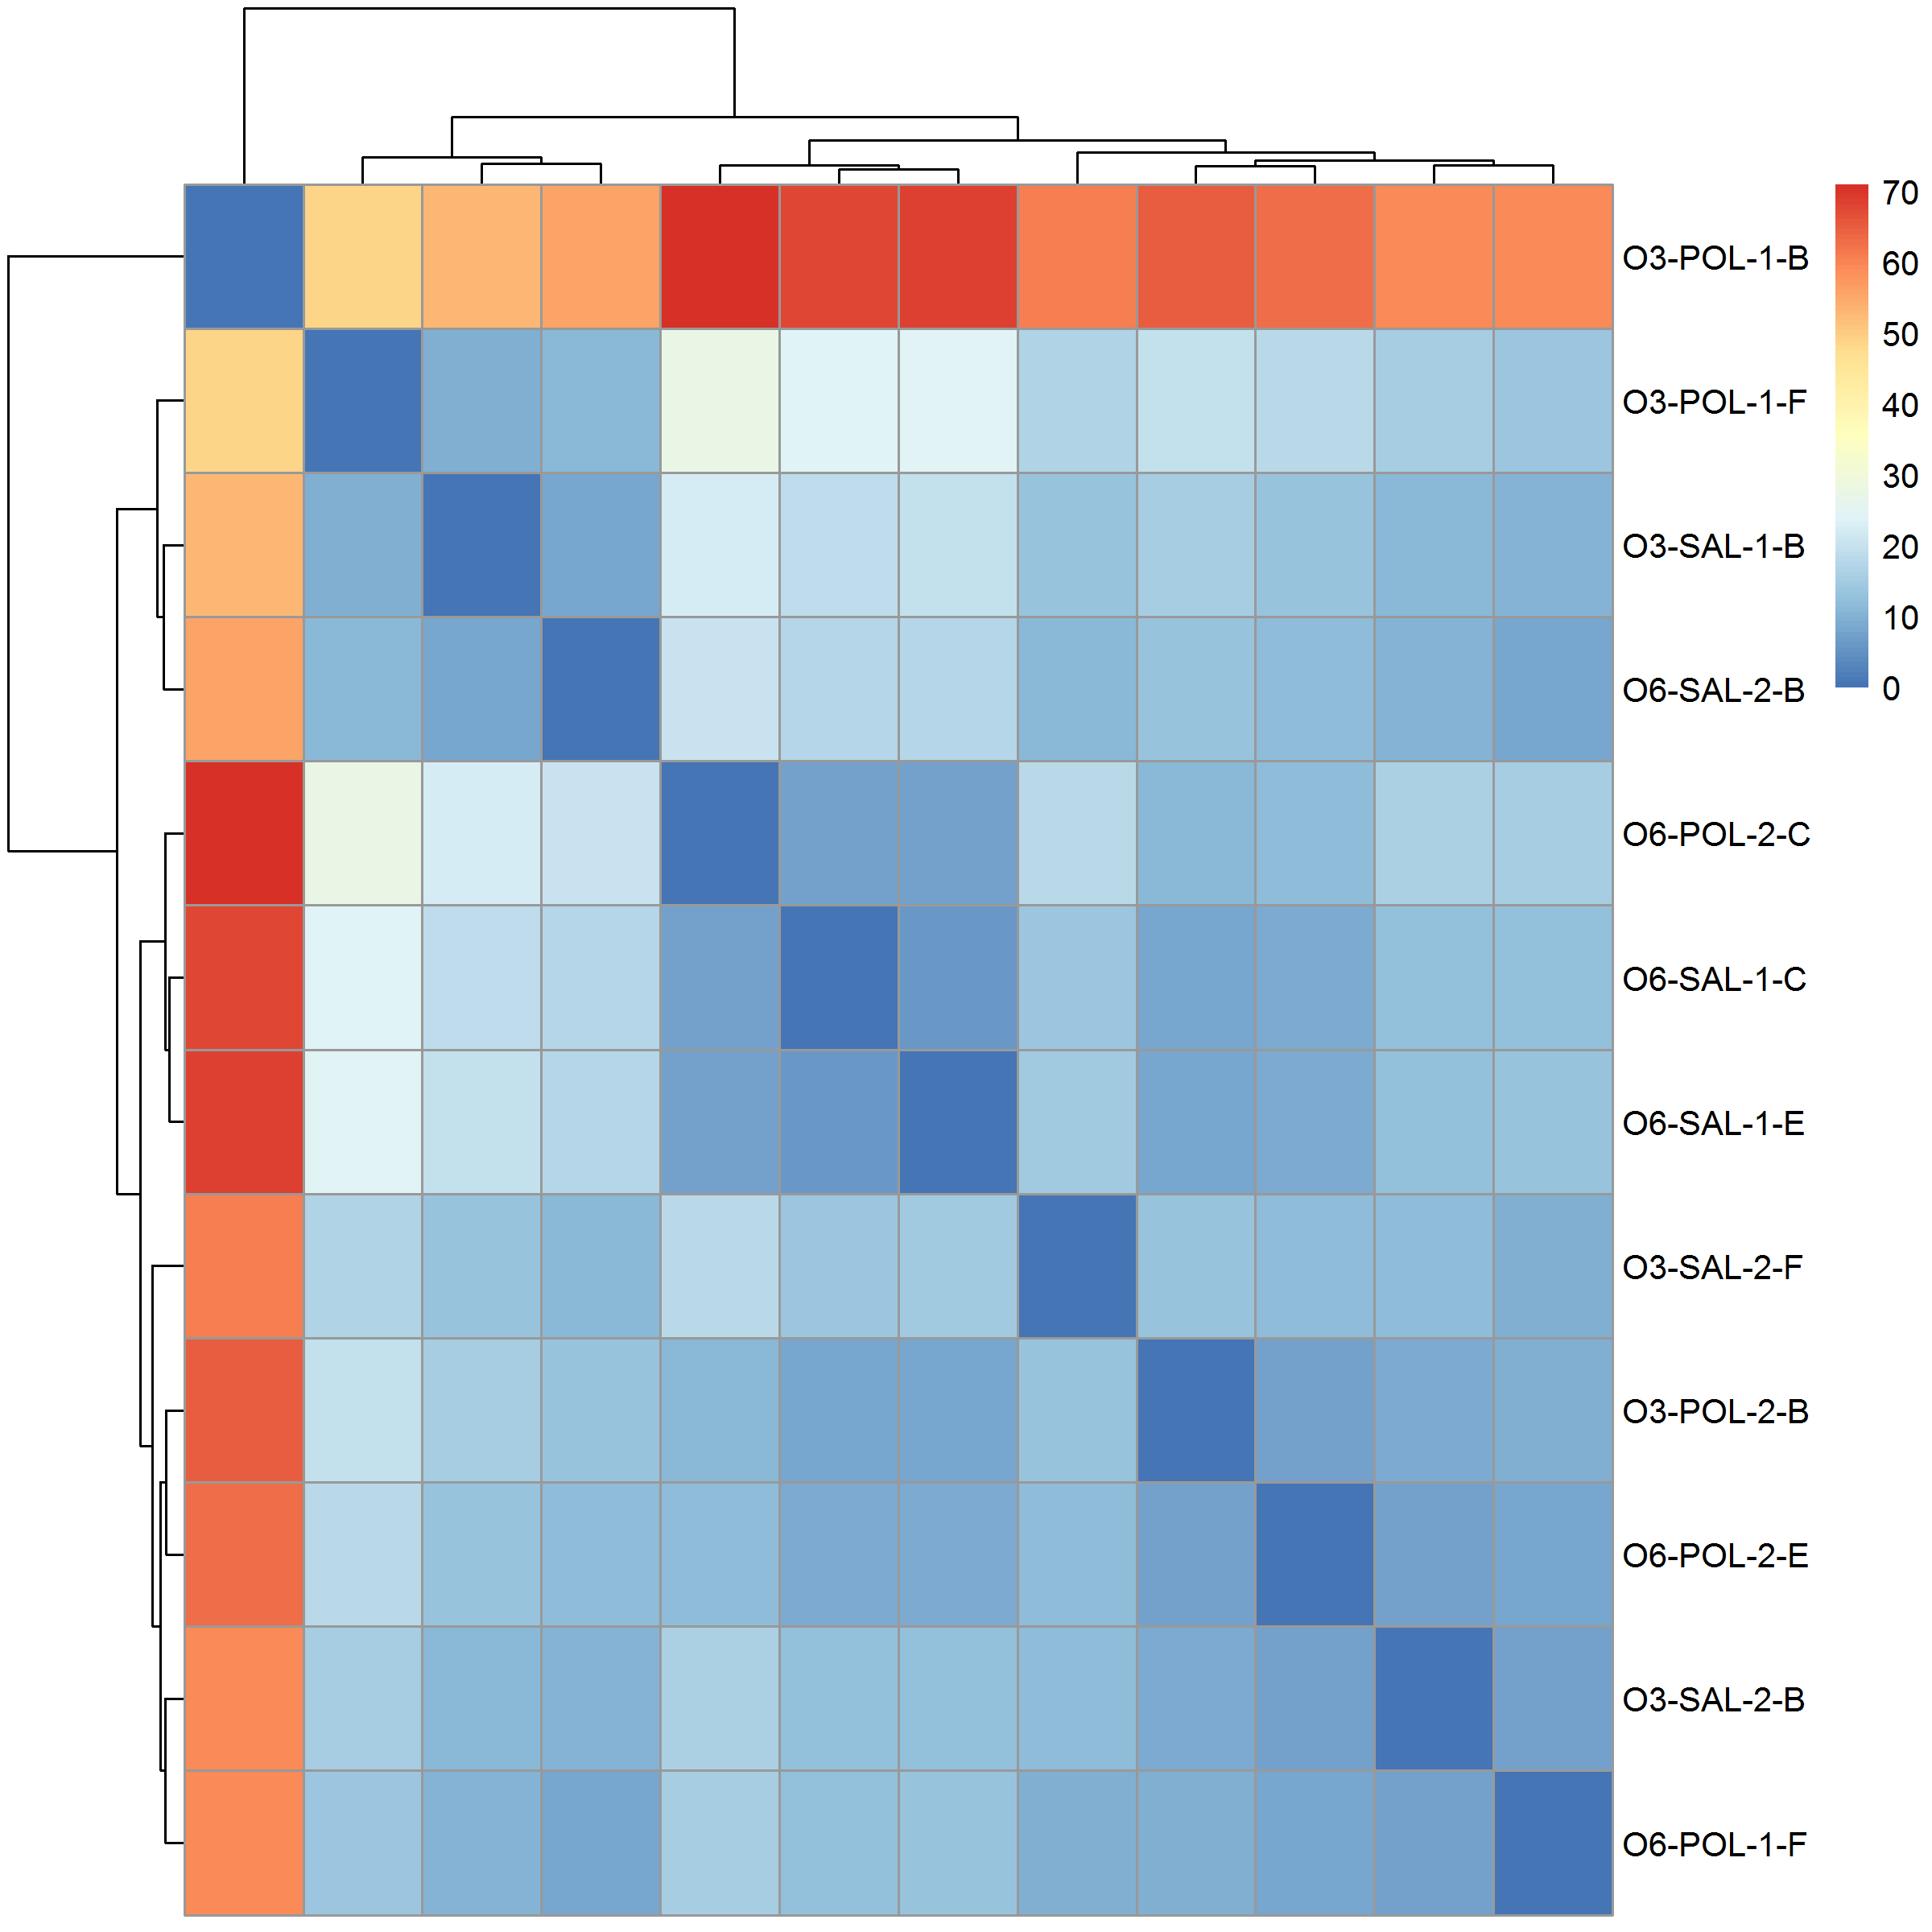
\includegraphics[width=\textwidth]{figure/DistanceMatrix.png}
	\caption[Sample Clustering]{Sample Clustering results.
		It was observed that there was no clear clustering for lane or batch effects.
		However, one sample from the Omega3-\gls{polyic} group was found to be substantially different from all other samples.
		
		It was unclear whether if the difference was due to sample contaminations or was due to sample mis-label.
		To avoid problems in down-stream analysis, we excluded this sample from subsequent analyses }
	\label{fig:distMatrix}
 \end{figure}

\subsubsection{Differential Expression Analysis}

\subsubsection{Functional Annotation}

\section{Discussion}